% !TEX root = Master.tex

In Section \ref{ssec:data_sources} we introduced the setup of the data to be treated. As one can see in \autoref{tab:article_master_data}, each article can be assigned to a set of attributes. Besides some elemental attributes like \textit{color}, \textit{age group} or \textit{gender}, the data exhibit a "natural" company-specific hierarchical structure. In \autoref{fig:article_hierarchy}, we can see an example of such a hierarchy for the attributes \textit{\ac{KCC}} and \textit{\ac{BS}} (See \autoref{tab:article_master_data}). The bottom level consists of the individual articles and at the top level we have the brand. It is important to mention that there are more inner levels between the brand and the articles than depicted in the Figure below. For example, \ac{KC} would be the level below \ac{KCC}. \acp{KCC} are aggregated sport/fashion categories and \acp{KC} add an additional layer to \acp{KCC}, namely the \textit{Product Division} covering Footwear, Apparel and Accessories/Hardware. The \ac{BS} supplements the \ac{KC} with a consumer driven "gender" perception.
Within the scope of this thesis, we will be concerned with the hierarchical structure of \autoref{fig:article_hierarchy} and in particular our \acp{KCC} of interest are \textit{"KCC 2"}, \textit{"KCC 6"} and \textit{"KCC 8"}.\footnote{Details on other structures in the appendix.}

\begin{figure}[H]
\centering
  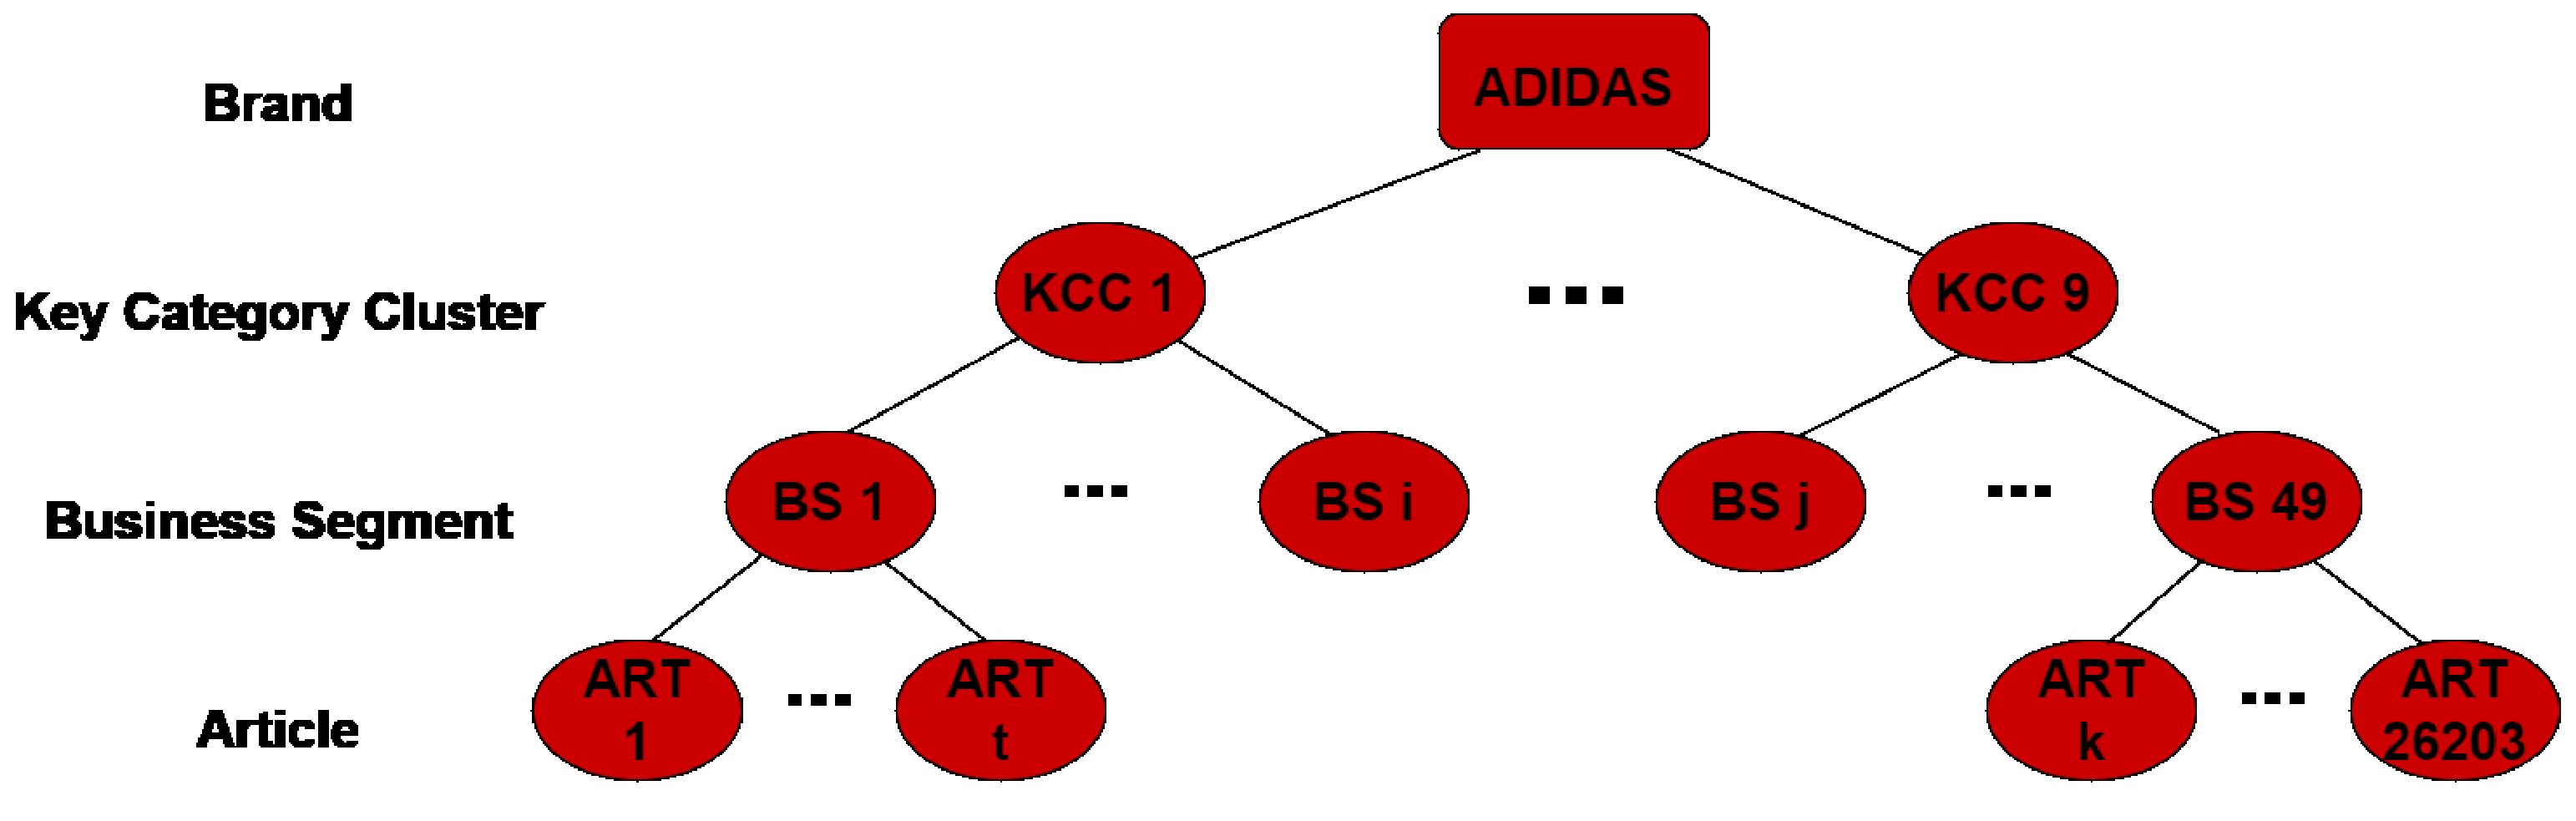
\includegraphics[width=0.95\linewidth]{figures/article_tree_KCC_BS.eps}
  \caption{Illustration of a hierarchical article structure}
  \label{fig:article_hierarchy}
\end{figure}

Worth mentioning is that it is possible that some individual nodes might have only one single child node, meaning that the hierarchy level can stay consistent across multiple nodes. This phenomenon however is very rare and when it occurs, it affects usually two consecutive nodes only. For example, \textit{Sub-Brand 4} has only one child node \textit{KCC 6} (See \autoref{fig:single_childnode}). Sub-Brands are visible for consumers through an own, not shared logo (See \autoref{fig:adidas_logos}).

\begin{figure}[H]
\centering
  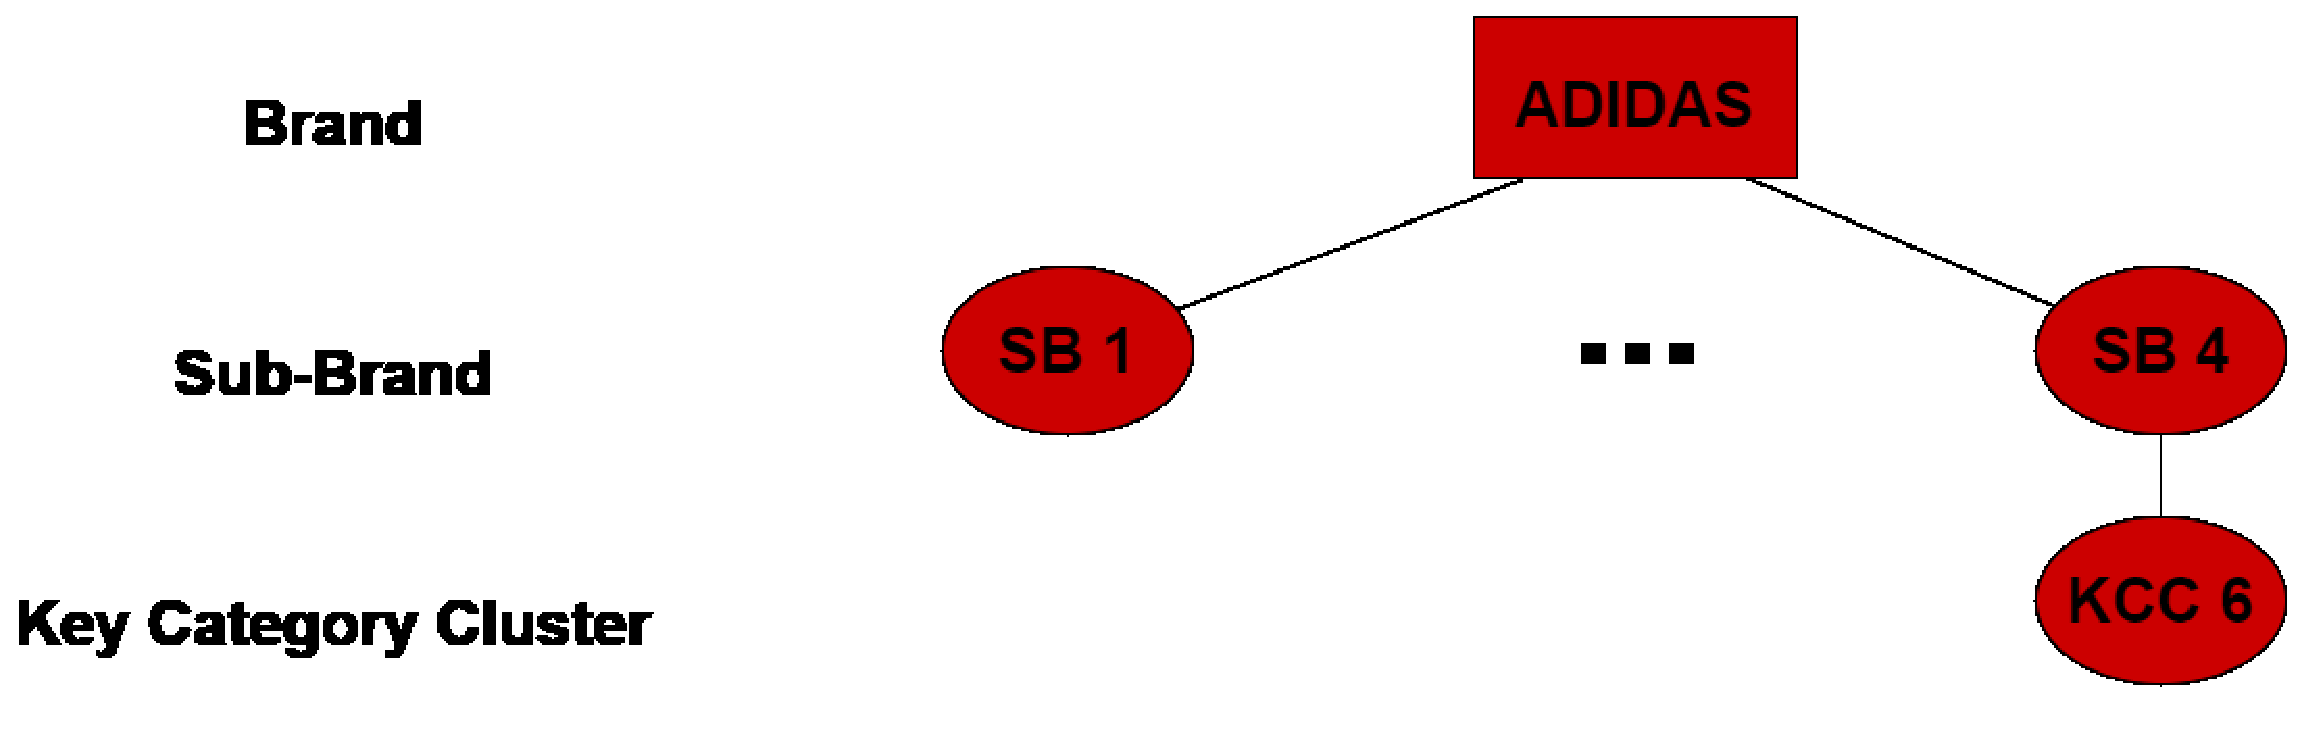
\includegraphics[width=.7\linewidth]{figures/article_tree_single_childnode.eps}
  \caption{Example of a single child node}
  \label{fig:single_childnode}
\end{figure} 

As mentioned in Section \autoref{ssec:data_sources}, our data contains the information about sold articles over the years 2017 and 2018. \autoref{fig:total_sold_articles_ts} shows the weekly course for the quantities over those two years, highlighting active promotion weeks as vertical lines. We can undoubtedly recognize that \textit{"Black Friday"} weeks have an exceptional impact on sales, as they stand internationally for the most busy shopping periods. During these days in mid- to late November each year, large amounts of different products are heavily discounted.

\begin{figure}[H]
\centering
  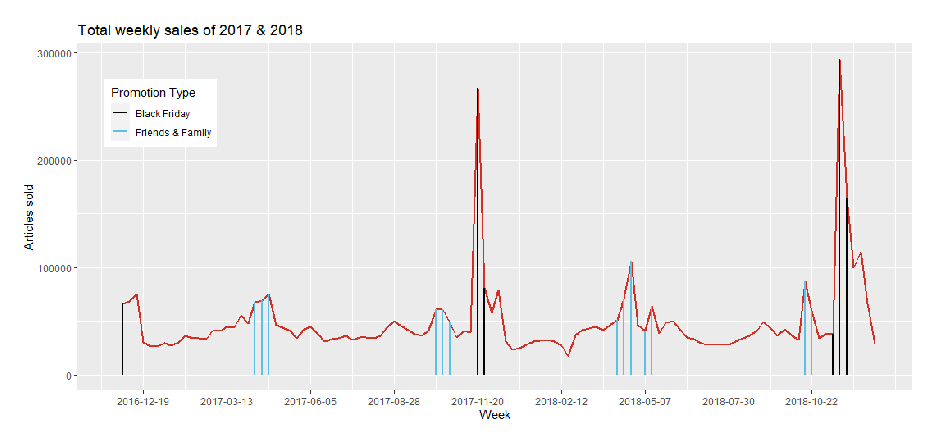
\includegraphics[width=1\linewidth]{figures/total_sold_articles_ts.eps}
  \caption{Total course of sold articles}
  \label{fig:total_sold_articles_ts}
\end{figure}

Another promotion type we are interested in is \textit{"Friends \& Family"}, occurring yearly around April-May and October, where on the eCom website plenty of articles are on offer. On these weeks, we have elevated numbers of sold articles as well(\autoref{fig:total_sold_articles_ts}). Tables \ref{tab:black_friday} and \ref{tab:friends_and_family} show the weeks were Black Friday and Friends \& Family took place respectively. The dates indicate always the Monday of the respective week (we assume that a week starts on Monday).


\begin{table}[H]
\setlength\arrayrulewidth{1pt}  
\centering
\begin{adjustbox}{max width=\textwidth}

\
\begin{tabular}{|
>{\columncolor{Gray}}c |c|c|c|c|c|c|}
\hline
\textbf{Black Friday weeks} & 2016-11-28 & 2017-11-20 & 2017-11-27 & 2018-11-12 & 2018-11-19 & 2018-11-26 \\ \hline
\end{tabular}

\end{adjustbox}
\caption{Black Friday weeks}
\label{tab:black_friday}
\end{table}



\begin{table}[H]
\setlength\arrayrulewidth{1pt}  
\centering
\begin{adjustbox}{max width=\textwidth}

\
\begin{tabular}{|
>{\columncolor{Gray}}c |c|c|c|c|c|c|c}
\hline
\cellcolor{Gray}                                              & 2017-04-10 & 2017-04-17 & 2017-04-24 & 2017-10-09 & 2017-10-16 & 2017-10-23 & \multicolumn{1}{l|}{2018-04-09} \\ \cline{2-8} 
\multirow{-2}{*}{\cellcolor{Gray}\textbf{Friends \& Family weeks}} & 2018-04-16 & 2018-04-23 & 2018-05-07 & 2018-05-14 & 2018-10-15 & 2018-10-22 &            \\ \cline{1-7}
\end{tabular}

\end{adjustbox}
\caption{Friends \& Family weeks}
\label{tab:friends_and_family}
\end{table}





